\chapter{Linguaggi}

\section{Introduzione}
Abbiamo visto, a partire dal capitolo relativo alla costruzione di HA, che si rende necessario 
definire un linguaggio con cui la macchina lavora. Dato un insieme $\Sigma$ di simboli
possiamo definire l'insieme $\Sigma^*$ di tutte le stringhe ottenute a partire da quei
simboli in maniera costruttiva
\[ nihl\in\Sigma^*\qquad a\in\Sigma , b\in\Sigma^*\Rightarrow a*b\in\Sigma^* \]
dove $nihl$ è la stringa vuota.

Un linguaggio $L$ è un sottoinsieme di $\Sigma^*$ definibile attraverso delle regole di
costruzione o anche solo attraverso l'enumerazione di tutte le stringhe che gli appartengono.
Ad esempio, se $\Sigma$ è costituito dalle lettere dell'alfabeto, maiuscole, minuscole, accentate,...
le stringhe appartenenti al linguaggio $I$ della lingua italiana sono facilmente, per modo di dire,
enumerabili in un dizionario. Un altro linguaggio che abbiamo visto è quello per la costruzione di
termini e formule in HA; certe espressioni non sono accettabili perchè sono prive di senso, ad esempio
la funzione successore applicata a due termini, $\forall\vee x$, insomma, espressioni non costruibili 
a partire dall'insieme $\Sigma$ tramite le regole di HA.

Che le regole di costruzione per un linguaggio siano molto importanti è facile capirlo anche
nell'ambito della programmazione informatica; sappiamo benissimo che se non scriviamo correttamente
un programma non solo ci potrebbe fare calcoli che non abbiamo chiesto, ma anche non lavorare proprio!

Un calcolatore è un programma che legge un programma scritto in linguaggio di programmazione (linguaggio
sorgente) e lo traduce in un programma equivalente (linguaggio oggetto) eseguibile da una macchina.
un utente può quindi eseguire il programma per passare da input ad output.

Tra le fasi di un calcolatore due in particolare ci interessano, l'analisi lessicale e l'analisi sintattica; nella prima
il calcolatore legge la stringa e raggruppa i caratteri in sequenze chiamati lexemi, a cui asoocia dei token, che 
contengono il nome del lexema e il valore attribuito; nella seconda fase, detta anche parsing, vengono usate le
prime parti del token per creare delle rappresentazione ad albero della lista dei token, che ci torna utile per
mostrare l'ordine in cui eseguire le operazioni.

Esempio: comando
[posizione = iniziale + velocità*60]
l'analisi lessicale creerà la stringa di token
[<id,1>,<=><id,2><+><id,3><*><60>]
dove per $id$ sta ad indicare la tavola dei simboli (alla posizione 1 c'è $posizione$), mentre l'analisi garmmaticale
creerà l'albero di parsing qui di seguito.
\begin{figure}[h]
	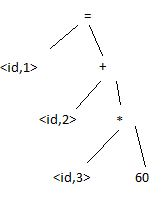
\includegraphics{img/Capture.JPG}
	\label{fig:Capture}
\end{figure}

Solitamente per l'analisi lessicale vengono usati lingauggi regolari, ovvero linguaggi che sono riconducibili ad automi
a stati finiti, mentre per l'analisi sintattica i lingauggi liberi da contesto, a cui si possono associare automi a pila o equivalentemente delle grammatiche. Ma come si possono classificare i linguaggi?
\begin{figure}[h]
	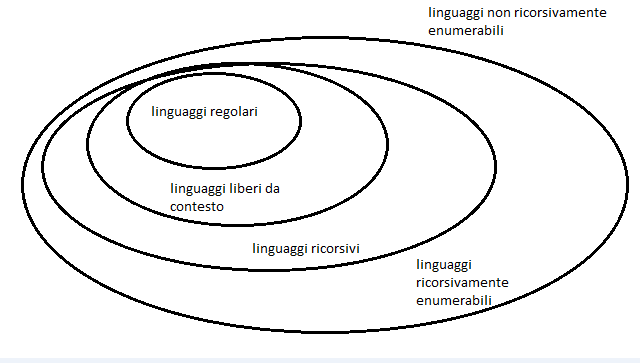
\includegraphics[width=0.75\textwidth]{img/liguaggi.png}
	\label{fig:liguaggi}
\end{figure}

Come visto nel capitolo 6, dato l'nsieme $\mathbb{N}$ dei numeri naturali esistono sottoinsiemi ricorsivi, ovvero
definibili da una funzione caratteristica associata,  insiemi ricorsivamente enumerabili, definibili da una funzione
semicaratteristica, e insiemi non ricorsivamente enumerabili, per i quali non esiste nessuna funzione semicaratteristica associabile. Il discorso può essere fatto analogamente per i linguaggi, che altro non sono che sottoinsiemi
dell'insieme $\Sigma^*$; visto che $\Sigma^*$ e $\{1\}^*\approx\mathbb{N}$  sono tra loro isomorfi, si può
parlare di lingauggi ricorsivi, r.e., non r.e..

Diciamo che una macchina di Turing $M$ accetta una stringa se, definito un sottoinsieme $F$ (stati di accettazione)tra gli stati della macchina $Q$ si ha che, data la stinga in input sul nastro, $M$ si arresta e termina in uno stato appartenente a $F$.
Se si arresta su uno stato appartenente a $Q/F$ si dice che la stringa non è accettata dalla macchina; e se non si arresta? Allora non possiamo dire nulla.

Data l'equivalenza tra fuzioni ricorsive totali o parziali con le macchine di Turing possiamo servirci delle macchine di Turing per definire i linguaggi. Un linguaggio $L$ si dice ricorsivo se esiste una $T_M$ che si arresta sia che la stringa appartenga al linguaggio, e quindi si arresta in uno stato di accettazione, sia che non appartenga al linguaggio, in uno stato non di accettazione. Un linguaggio $L$ è r.e. se la $T_M$ associata si ferma quando accetta la stringa ma va in loop, ovvero non si arresta, quando non accetta la stringa. Un linguaggio è non r.e. se non si può nemmeno definire una macchina di Turing per tale liguaggio.

I linguaggi regolari e quelli liberi da contesto ,visti prima, sono linguaggi la cui macchina di Turing associata assume caratteristiche più semplici rispetto ad una macchina di Turing. Ad esempio, i linguaggi regolari sono associabili ad automi a stati finiti, che altro non sono che macchine di Turing su cui non si può tornare indietro e sulle quali non si può sovrascrivere nulla.

Esempio $L=\{w\in{0,1}^*,0,1$ alternati in $w\}$. Possiamo associare a $L$ il seguente automa
\begin{figure}[h]
	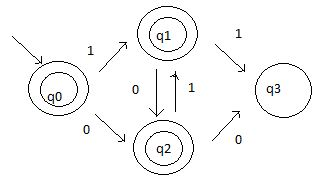
\includegraphics[width=0.35\textwidth]{img/automa.JPG}
	\label{fig:Capture}
\end{figure} 

dove gli stati di accettazione sono cechiati (ovviamente, anche la stinga vuota appartiene a questo linguaggio!).

Per i linguaggi liberi da contesto si possono usare automi a pila o equivalentemente grammatiche per costruire alberi di parsing, come visto sopra. Esempio $L_{pal}$ è l'insieme delle stringhe palindromi, ovvero che lette al contrario sono uguali.
Una grammatica che funziona è questa
\[P->\epsilon|0|1|0P0|1P1\]
ovvero dato un nodo $P$ lo possiamo potare, ovvero mandarlo nella striga vuota, sostituire con $0$ o $1$ , oppure con due foglie uguali (o $0$ o $1$) e un nodo $P$ in mezzo. Risulta facile costruire un albero a partire dal nodo iniziale $P$.

Ci sono delle condizioni necessarie per dire se un linguaggio è regolare o libero da contesto; purtroppo sono condizioni necessarie ma non sufficienti. Non solo, come abbiamo avuto occasione di vedere a lezione, anche solo decidere se un linguaggio è ricorsivamente enumerabile, o trovare una macchina di Turing che lo accetti, è no banale; in generale, per il teorema di Rice (capitolo 2) ogni proprietà non banale di un linguaggio è indecidibile.

\subsection{Esempi di linguaggi}
 
Abbiamo visto nel capitolo 3 esempi di macchine di Turing che fanno calcoli, quali somma, prodotto, differenza, etc. Vediamo di seguito una macchina di Turing che riconosce il linguaggio ricorsivo $L=\{o^n1^n, n>0\}$.
\begin{figure}[h]
	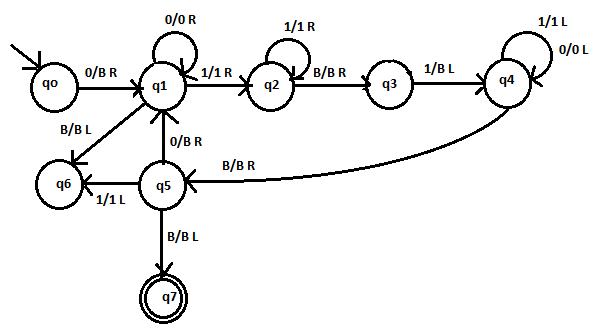
\includegraphics[width=0.70\textwidth]{img/turing.png}
	\label{fig:Capture}
\end{figure} 
 
La macchina di Turing riconoscerà se la stringa appartiene o meno al linguaggio se si ferma allo stato $q7$, altrimenti si può facilmente notare che la macchina si ferma comunque.

Un esempio di lingauggio che è r.e. ma non ricorsivo è dato dal linguaggio universale $L_U=\{(M,w)|w\in L(M)\}$, dove $M$ è la codifica binaria di una macchina di Turing e w una stringa qualsiasi, e $L(M)$ è l'insieme delle stringhe che una macchina di Turing accetta.; in pratica $L_U$ è l'insieme di tutte le copie di $T_M$  e di stringhe accettate dalla $T_M$. Ma dire se una stringa è accettata o meno da una $T_M$ qualsiasi equivale al classico problema dell'arresto, ed è una proprietà non banale di un linguaggio, quindi non decidibile. Nel capitolo 2 si può trovare una codifica effettiva della macchina di Turing Universale $UTM$, con $L(UTM)=L_U$.

Vediamo ora un linguaggio che non è nemmeno r.e.. Sappiamo che possiamo ordinare lessicograficamente e per lunghezza le stringhe di un linguaggio, e analogamente i codici delle macchine di Turing; ad ogni $i\in\mathbb{N}$ possiamo pertanto associare una stringa $w_i$ e una macchina $M_i$. Dopo queste premesse definiamo il seguente linguaggio (diagonale)
\[ L_D=\{w_i\in\Sigma^*|w_i\notin L(M_i)\}\].
Se il linguaggio $L_D$ fosse r.e. potremmo associargli una macchina $M_D$ che lo accetta. Sappiamo che se $w_i\notin L(M_i)$, allora $w_i\in L(M_D)$. Ma $D$ risulterà essere un numero naturale, perchè tutte le macchina di Turing sono ordinabili; esisterà quindi anche un $w_D$ analogamente a $M_D$. Ora se $w_D\in L(M_D)$, allora essendo $w\in L_D=L(M_D)$, si dovrebbe avere, per definizione di linguaggio diagonale, che $w_D\notin L(M_D)$ , e viceversa se $w\in L(M_D)$ allora $w\notin L(M_D)$. L'assurdo discende dall'aver assunto che esistesse una tale $M_D$.

Vediamo ora due ulteriori esempi di linguaggio che sono tra loro chiaramente complementari
\[L_e=\{M|L(M)=\emptyset\}\]\[L_{ne}=\{M|L(M)\neq\emptyset\}\].
Facciamo vedere che $L_{ne}$ è r.e., mostrando che esiste una $T_M$ che lo accetta. Basta prendere una $M$ non deterministica che, data $M_i$ in imput, non deterministicamente simuli $M_i$ su tutte le possibili $w$. Se c'è una $w$ che è accettata da $M_i$, allora $M$ accetta $M_i$.

Per mostrare che invece $L_{ne}$ non è ricorsivo, operiamo una riduzione dal $L_U$ a $L_{ne}$. Visto che $L_U$ non è ricorsivo, non lo può essere nemmeno $L_{ne}$; se invece si assumesse che $L_{ne}$ fosse ricorsivo, anche $L_U$ dovrebbe esserlo, e si avrebbe un assurdo.

Per la riduzione, dobbiamo associare ad ogni coppia $(M,w)$ con $w\in L(M)$ una macchina di Turing $M'$ tale che $w\in L(M)$ se e solo se $L(M')\neq\emptyset$. $M'$ è una $T_M$ che ignora il suo imput e simula $M$ su $w$. Se $M$ accetta $w$, allora $M'$ accetta il suo imput, pertanto $L(M')\neq\emptyset$. Se $M$ non accetta $w$, allora $M'$ non accetta nessun imput, quindi $L(M')=\emptyset$.

Ora per il teorema 6.9, essendo $L_e$ il complementare di $L_{ne}$, se $L_e$ fosse r.e., sia $L_e$ che $L_{ne}$ dovrebbero essere ricorsivi. Ma abbiamo già visto che non è così. Quindi $L_e$ non è nemmeno r.e..

